\documentclass[a4paper,10pt]{article}
\usepackage{amsfonts, amssymb, amsmath, graphicx, float, subfigure}
\title{Dynamical Matching in a Caldera Potential Energy surface} 
\author{Matthaios Katsanikas}
\begin{document}
                           
\maketitle

\section{The Model} 

Dynamical matching is an interesting mechanism originally proposed in \cite{carpenter1985,carpenter1995} that arises in Caldera-type potential energy surfaces (PES). These potentials are relevant in Chemistry since they provide good approximations for many organic chemical reactions such as those that occur in the vinylcyclopropane-cyclopentene rearrangement \cite{baldwin2003,gold1988}, the stereomutation of cyclopropane \cite{doubleday1997}, the degenerate rearrangement of bicyclo[3.1.0]hex-2-ene \cite{doubleday1999,doubleday2006} or that of 5-methylene\\bicyclo[2.1.0]pentane \cite{reyes2002}. The potential energy landscape of a Caldera is similar to that of a collapsed region in an erupted volcano. It is characterized by a shallow potential well region (a central minimum) surrounded by four entrance/exit channels in the form of index-1 saddles. Two of these saddles have low energy values and correspond to the formation of chemical products, while the other two are higher in energy and represent reactants. The dynamical matching phenomenon occurs when the Newtonian momentum conservation will favor that a trajectory entering the Caldera from a channel corresponding to a high energy index-1 saddle (reactant) exits through the diametrically opposing low energy index-1 saddle (product). Consequently, this mechanism will determines to a considerable extent the outcome of the chemical reaction.

\begin{figure}[htbp]
	\centering
	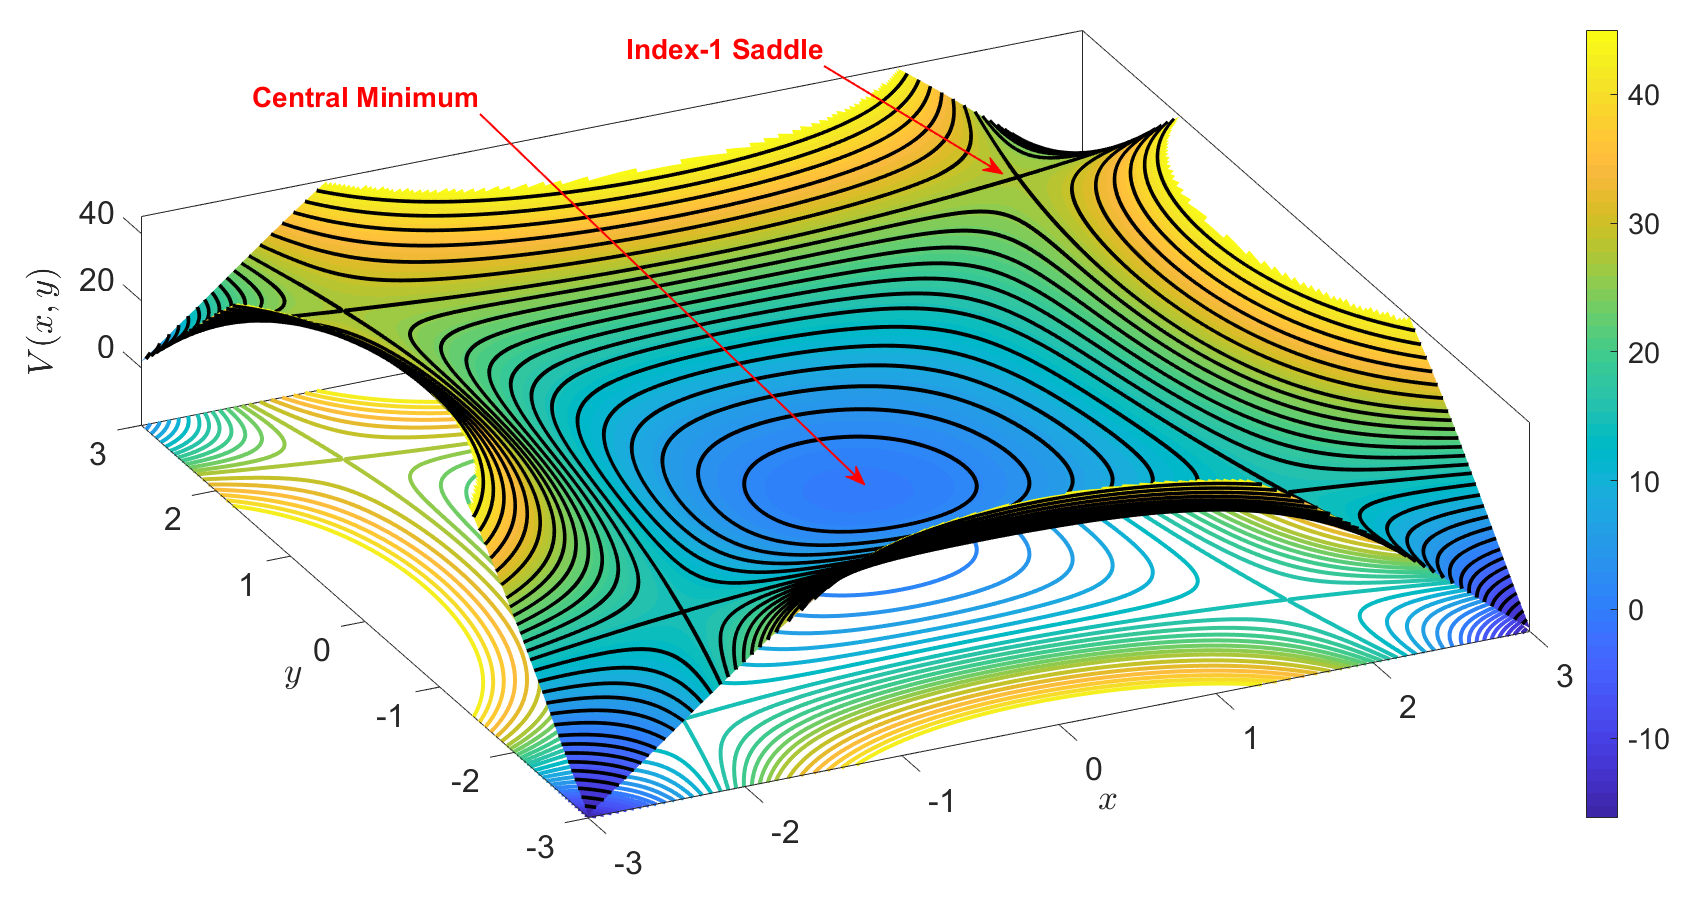
\includegraphics[scale=0.25]{caldera_pes_lambda_1.png}
	\caption{Caldera potential energy surface given by Eq. (\ref{eq1}) for the model parameters $c_1 = 5$, $c_2 = 3$, $c_3 = -3/10$ and $\lambda = 1$.}
	\label{caldera_pes}
\end{figure}


\bibliographystyle{plain}
\bibliography{caldera2c}




\end{document}


